\documentclass[12pt,a4paper]{article}

\usepackage[utf8]{inputenc}
\usepackage[T1]{fontenc}
\usepackage[slovene]{babel}
\usepackage{lmodern}
\usepackage[a4paper,margin=2.5cm]{geometry}
\usepackage{setspace}
\usepackage{indentfirst}
\usepackage{parskip}
\usepackage{amsmath}
\usepackage{amssymb}
\usepackage{amsthm}
\usepackage{mathtools}
\usepackage{graphicx}
\usepackage{float}
\usepackage{subcaption}
\usepackage{booktabs}
\usepackage{array}
\usepackage{multirow}
\usepackage{longtable}
\usepackage{makecell}
\usepackage{xcolor}
\usepackage{enumitem}
\usepackage{listings}
\usepackage[hidelinks]{hyperref}
\usepackage{caption}
\captionsetup[figure]{font=small}
\captionsetup[table]{font=small}

\onehalfspacing

\setlength{\parindent}{1.25cm}
\setlength{\parskip}{0.3em}

\graphicspath{{img/}}
\begin{document}
\title{Analiza vpliva geometrijskih odmikov QCA celic na delovanje in
odpornost večinskih logičnih vrat}
\author{Blažič Teja, Čeh Nejc}
\maketitle


\abstract{
V seminarski nalogi raziskujemo vpliv geometrijskih odmikov kvantnih celičnih avtomatov (QCA) na delovanje večinskih logičnih vrat. Primerjamo osnovna petcelična večinska vrata in alternativna vrata, odporna na določene vrste napak,
ki so jih predstavili Wang in sodelavci. S simulacijami v programu QCADesigner-E analiziramo odmike posameznih celic v različnih smereh ter spremljamo pravilnost logične funkcije in izhodno polarizacijo.
Dodatno analiziramo spremembe elektrostatičnih interakcij pri premikanju osrednje celice osnovnih vrat. Rezultati kažejo, da so manjši odmiki praviloma manj problematični, medtem ko lahko večji odmiki povzročijo
nepravilno delovanje. Pri Wangovih vratih opazimo večjo odpornost notranjih celic, medtem ko so premiki vhodnih in izhodne celice lahko občutljivejši. Ugotovitve poudarjajo pomen geometrijske razporeditve
celic pri načrtovanju odpornih QCA vezij. }

\section{Uvod}
\label{g18:sec:uvod}

Kvantni celični avtomati (QCA) predstavljajo alternativni pristop k načrtovanju logičnih vezij, pri katerem se informacija prenaša
z elektrostatičnimi interakcijami med sosednjimi celicami. Eden osnovnih gradnikov QCA vezij so večinska logična vrata, ki izvajajo funkcijo

\begin{equation}
    M(A,B,C) = AB + AC + BC.
    \label{g18:eq:majority}
\end{equation}

Zaradi majhnih dimenzij QCA celic lahko že manjši geometrijski odmiki vplivajo na njihove medsebojne interakcije in posledično na pravilnost delovanja vezja. Zato je odpornost na tovrstne napake pomembna pri načrtovanju QCA struktur.

V seminarski nalogi analiziramo vpliv geometrijskih odmikov na osnovna petcelična večinska vrata in alternativna vrata,
ki so jih predstavili Wang in sodelavci~\cite{g18:wang2018}. Slednja so zasnovana za večjo odpornost na določene napake, predvsem na manjkajoče
celice. Zanima nas, ali so odporna tudi na spremembe položajev posameznih celic.

\textbf{Raziskovalno vprašanje:}Kako velikost, smer in položaj geometrijskega odmika posamezne QCA celice vplivajo na pravilnost delovanja osnovnih in Wangovih večinskih vrat?

\textbf{Pričakovani rezultati:}Pričakujemo, da bodo manjši odmiki večinoma ohranili pravilno delovanje, večji pa povzročili več napak.
Predvidevamo tudi, da bodo Wangova vrata odpornejša na odmike notranjih celic kot na odmike vhodnih in izhodne celice.

V nadaljevanju predstavimo uporabljene metode in simulacijske nastavitve, rezultate obeh struktur ter matematično analizo
elektrostatičnih interakcij. Rezultate nato interpretiramo in primerjamo s pričakovanji.


\section{Metode}
\label{g18:sec:metode}

\subsection{Orodja in nastavitve}
\label{g18:sec:orodja}

Za izdelavo in simulacijo vezij smo uporabili program QCADesigner-E. Osnovna večinska vrata so sestavljena
iz petih celic dimenzije $18 \times 18$ nm, razdalja med središči sosednjih celic pa znaša 20 nm.

Za spremljanje polarizacije in analizo elektrostatičnih interakcij smo uporabili simulacije, pri katerih smo
med posameznimi poskusi spreminjali samo položaj izbrane celice. Ostali parametri so ostali nespremenjeni.

\begin{table}[htbp]
    \caption{Osnovni parametri simulacij.}
    \label{g18:tab:parametri}
    \centering
    \begin{tabular}{ll}
        \toprule
        Parameter & Vrednost \\
        \midrule
        Program & QCADesigner-E \\
        Model & Coherence Vector with Energy \\
        Dimenzije celice & $18 \times 18$ nm \\
        Razdalja med središči & 20 nm \\
        \bottomrule
    \end{tabular}
\end{table}


\subsection{Zasnova poskusov}
\label{g18:sec:poskusi}

Raziskavo smo izvedli na dveh različnih strukturah večinskih vrat.

\subsubsection{Osnovna petcelična vrata}

Najprej smo implementirali osnovna večinska vrata s tremi vhodnimi celicami $A$, $B$ in $C$, osrednjo celico ter izhodno celico $Y$.

Posamezne celice smo premikali v štirih smereh: levo, desno, gor in dol. Pri različnih velikostih
odmikov smo spremljali pravilnost logične funkcije in polarizacijo izhodne celice.

\subsubsection{Wangova večinska vrata}

V drugem delu smo analizirali alternativno strukturo večinskih vrat, ki so jo predstavili Wang in sodelavci.

Preizkusili smo geometrijske odmike izbranih notranjih celic, vhodnih celic in izhodne celice. Pri tem smo
preverjali, kako posamezni odmiki vplivajo na pravilnost delovanja in izhodno polarizacijo.

\subsubsection{Energijska analiza}

Za podrobnejšo razlago vpliva odmikov smo analizirali elektrostatične interakcije med osrednjo in sosednjimi celicami osnovnih večinskih vrat.

Iz energijskih izpisov programa QCADesigner-E smo pridobili interakcijske koeficiente $E_k$ pri različnih položajih osrednje celice ter primerjali njihove spremembe.


\subsection{Metrike}
\label{g18:sec:metrike}

Pravilnost delovanja smo določili s preverjanjem vseh osmih kombinacij treh vhodnih logičnih vrednosti.
Za vsako kombinacijo smo izhodno polarizacijo primerjali s pričakovano vrednostjo večinske funkcije.
Pravilnost smo zapisali kot število pravilnih kombinacij od osmih, pri čemer $8/8$ pomeni popolnoma pravilno delovanje.

Poleg pravilnosti smo spremljali absolutno vrednost izhodne polarizacije $|P_Y|$. Ta predstavlja velikost polarizacije izhodne celice, 
ne pa tudi pravilnosti logične funkcije, saj je lahko celica močno polarizirana v napačno smer.

Pri energijski analizi osnovnih vrat smo dodatno spremljali interakcijske koeficiente $E_k$, ki jih podaja QCADesigner-E. Njihove spremembe pri različnih
geometrijskih odmikih bomo podrobneje obravnavali v razdelku~\ref{g18:sec:rez-energija}.

Za vrednost $|P_Y|$ smo uporabili absolutno vrednost največje oziroma najmanjše izhodne polarizacije, saj sta bili ti vrednosti nasprotno enaki.

\section{Rezultati}
\label{g18:sec:rezultati}

\subsection{Osnovna petcelična večinska vrata}
\label{g18:sec:rez-osnovna}

\subsubsection{Izhodiščna izvedba}

V programu QCADesigner-E smo sestavili petcelična večinska vrata s tremi vhodnimi celicami $A$, $B$ in $C$, osrednjo celico $M$
in izhodno celico $Y$. Postavitev in simulacijski prikaz izhodiščnega vezja sta prikazana na slikah
\ref{g18:fig:rez-osnovna-implementacija} in \ref{g18:fig:rez-osnovna-signali}.

\begin{figure}[H]
    \centering
    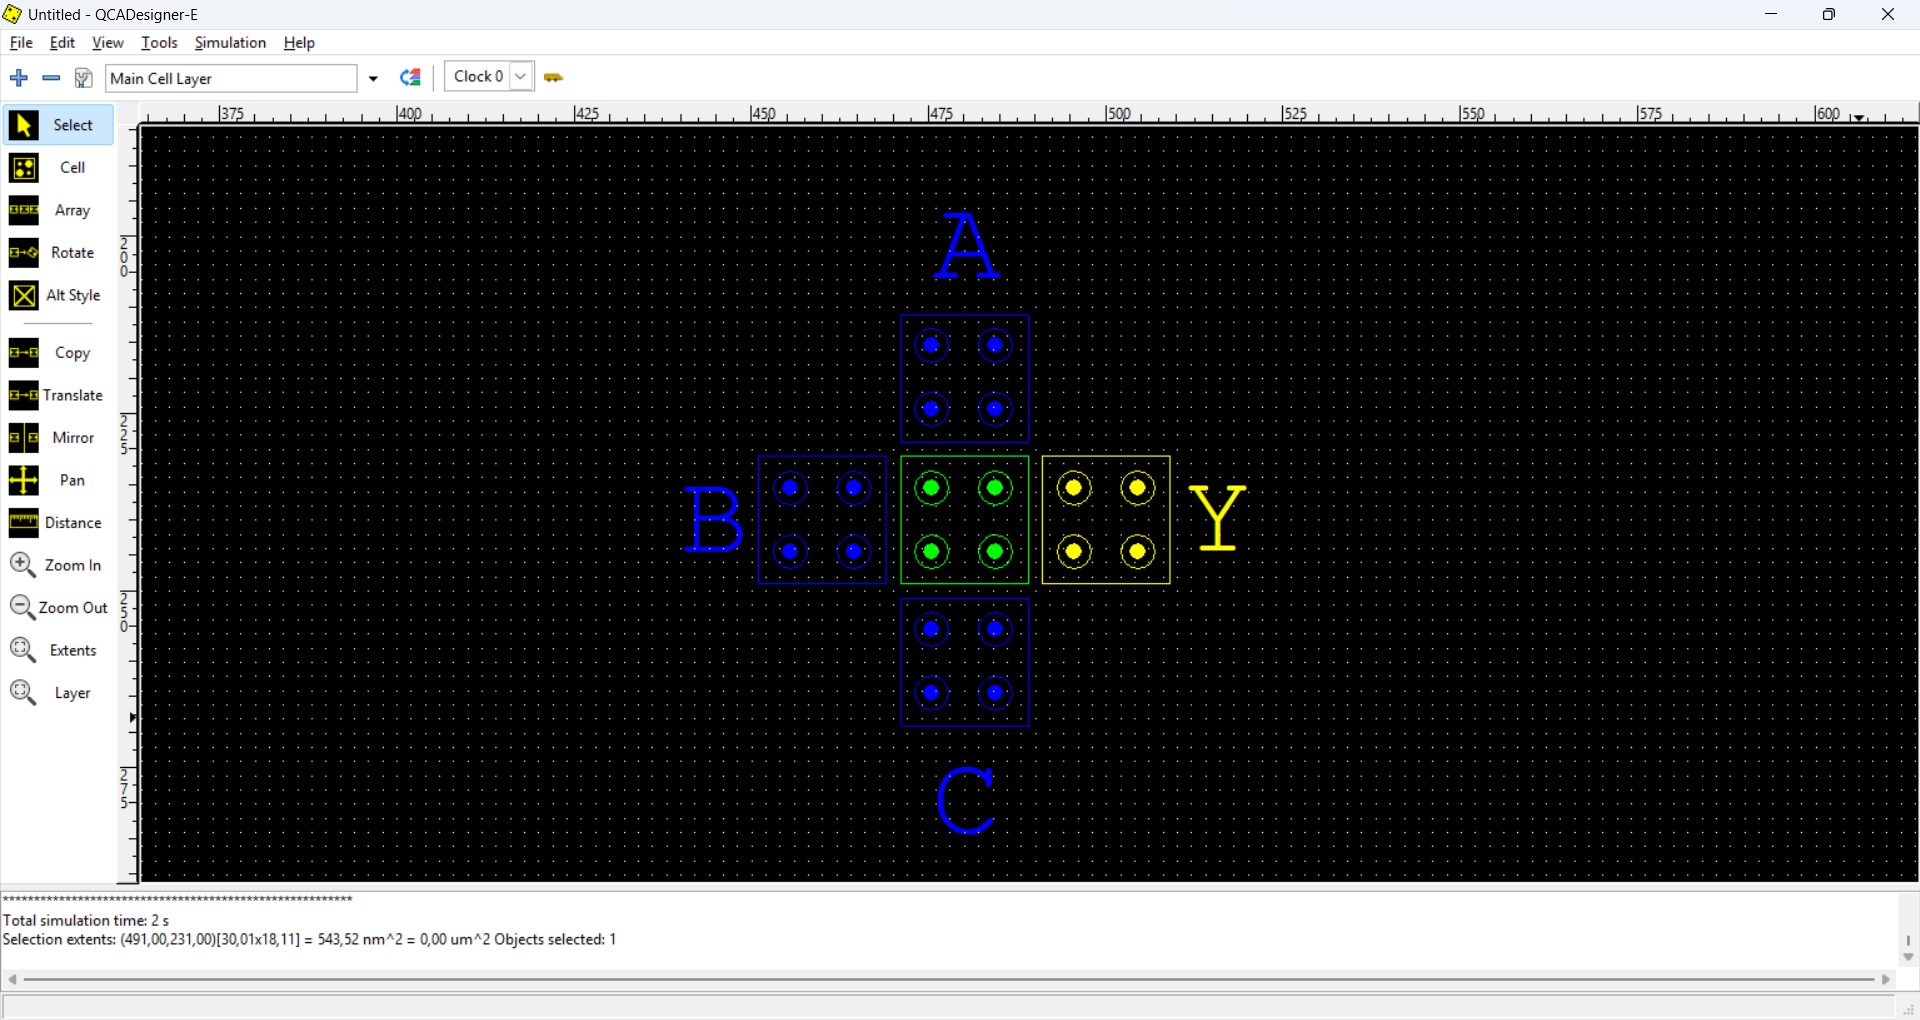
\includegraphics[width=0.82\textwidth]{vecinska_vrata_QCAD.png}
    \caption{Implementacija osnovnih petceličnih večinskih vrat v QCADesigner-E.}
    \label{g18:fig:rez-osnovna-implementacija}
\end{figure}

\begin{figure}[H]
    \centering
    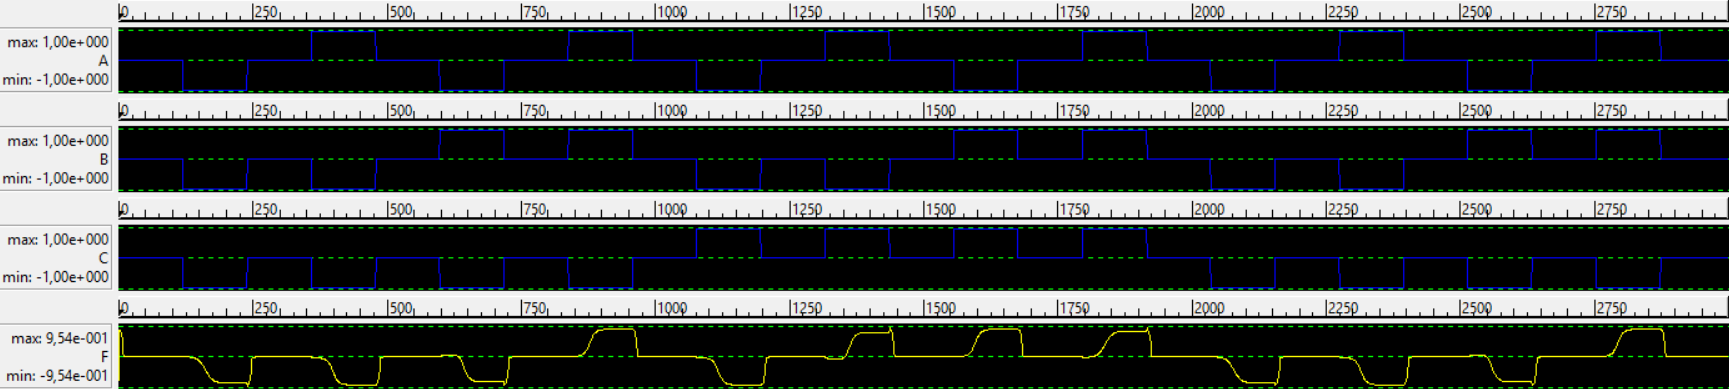
\includegraphics[width=0.82\textwidth]{vecinska_vrata_QCAD_rezultati.png}
    \caption{Simulacijski prikaz vhodnih signalov in izhodne polarizacije osnovnih večinskih vrat brez odmika.}
    \label{g18:fig:rez-osnovna-signali}
\end{figure}

Brez geometrijskih odmikov je vezje pravilno izvedlo vseh osem kombinacij vhodov ($8/8$); zabeležena absolutna izhodna polarizacija je bila $|P_Y|=0{,}954$.


\subsubsection{Rezultati geometrijskih odmikov}
\label{g18:sec:rez-osnovna-premiki}


Pri poskusih smo premikali le eno celico ter si beležili pravilnost logične funkcije in izhodno polarizacijo. Rezultati so prikazani v tabeli~\ref{g18:tab:osnovna-io}.

\begin{table}[H]
    \centering
    \captionsetup{font=small}

    \begin{minipage}{0.49\textwidth}
        \centering
        \resizebox{\linewidth}{!}{%
            \begin{tabular}{|c|c|c|c|c|}
                \hline
                Celica & Smer & Odmik [nm] & Pravilne kombinacije & $|P_Y|$ \\
                \hline
                A & Desno & 0.5 & 8/8 & 9.55e-001 \\
                A & Desno & 2.5 & 8/8 & 9.60e-001 \\
                A & Desno & 5.0 & 6/8 & 9.76e-001 \\
                A & Desno & 10.0 & 4/8 & 9.76e-001 \\
                A & Desno & 50.0 & 6/8 & 9.68e-001 \\
                A & Levo & 0.5 & 8/8 & 9.55e-001 \\
                A & Levo & 2.5 & 8/8 & 9.59e-001 \\
                A & Levo & 5.0 & 8/8 & 9.62e-001 \\
                A & Levo & 10.0 & 4/8 & 9.69e-001 \\
                A & Levo & 50.0 & 6/8 & 9.66e-001 \\
                A & Gor & 0.5 & 8/8 & 9.55e-001 \\
                A & Gor & 2.5 & 8/8 & 9.58e-001 \\
                A & Gor & 5.0 & 6/8 & 9.69e-001 \\
                A & Gor & 10.0 & 6/8 & 9.68e-001 \\
                A & Gor & 50.0 & 6/8 & 9.66e-001 \\
                A & Dol & 0.5 & 8/8 & 9.55e-001 \\
                A & Dol & 1.0 & 8/8 & 9.56e-001 \\
                A & Dol & 1.5 & 8/8 & 9.57e-001 \\
                A & Dol & 2.0 & 8/8 & 9.57e-001 \\
                \hline
            \end{tabular}
        }
    \end{minipage}
    \hfill
    \begin{minipage}{0.49\textwidth}
        \centering
        \resizebox{\linewidth}{!}{%
            \begin{tabular}{|c|c|c|c|c|}
                \hline
                Celica & Smer & Odmik [nm] & Pravilne kombinacije & $|P_Y|$ \\
                \hline
                B & Desno & 0.5 & 8/8 & 9.54e-001 \\
                B & Desno & 1.0 & 8/8 & 9.55e-001 \\
                B & Desno & 1.5 & 8/8 & 9.55e-001 \\
                B & Desno & 2.0 & 6/8 & 9.74e-001 \\
                B & Levo & 0.5 & 8/8 & 9.54e-001 \\
                B & Levo & 2.5 & 8/8 & 9.52e-001 \\
                B & Levo & 5.0 & 8/8 & 9.51e-001 \\
                B & Levo & 10.0 & 8/8 & 9.50e-001 \\
                B & Levo & 50.0 & 8/8 & 9.48e-001 \\
                B & Gor & 0.5 & 8/8 & 9.54e-001 \\
                B & Gor & 2.5 & 8/8 & 9.54e-001 \\
                B & Gor & 5.0 & 8/8 & 9.53e-001 \\
                B & Gor & 10.0 & 4/8 & 9.48e-001 \\
                B & Gor & 50.0 & 4/8 & 9.48e-001 \\
                B & Dol & 0.5 & 8/8 & 9.54e-001 \\
                B & Dol & 2.5 & 8/8 & 9.54e-001 \\
                B & Dol & 5.0 & 8/8 & 9.53e-001 \\
                B & Dol & 10.0 & 4/8 & 9.48e-001 \\
                B & Dol & 50.0 & 4/8 & 9.48e-001 \\
                \hline
            \end{tabular}
        }
    \end{minipage}

    \vspace{0.3cm}

    \begin{minipage}{0.49\textwidth}
        \centering
        \resizebox{\linewidth}{!}{%
            \begin{tabular}{|c|c|c|c|c|}
                \hline
                Celica & Smer & Odmik [nm] & Pravilne kombinacije & $|P_Y|$ \\
                \hline
                C & Desno & 0.5 & 8/8 & 9.55e-001 \\
                C & Desno & 2.5 & 8/8 & 9.60e-001 \\
                C & Desno & 5.0 & 6/8 & 9.76e-001 \\
                C & Desno & 10.0 & 4/8 & 9.76e-001 \\
                C & Desno & 50.0 & 6/8 & 9.68e-001 \\
                C & Levo & 0.5 & 8/8 & 9.55e-001 \\
                C & Levo & 2.5 & 8/8 & 9.59e-001 \\
                C & Levo & 5.0 & 8/8 & 9.62e-001 \\
                C & Levo & 10.0 & 4/8 & 9.69e-001 \\
                C & Levo & 50.0 & 6/8 & 9.66e-001 \\
                C & Gor & 0.5 & 8/8 & 9.55e-001 \\
                C & Gor & 1.0 & 8/8 & 9.56e-001 \\
                C & Gor & 1.5 & 8/8 & 9.57e-001 \\
                C & Gor & 2.0 & 8/8 & 9.57e-001 \\
                C & Dol & 0.5 & 8/8 & 9.55e-001 \\
                C & Dol & 2.5 & 8/8 & 9.58e-001 \\
                C & Dol & 5.0 & 6/8 & 9.69e-001 \\
                C & Dol & 10.0 & 6/8 & 9.68e-001 \\
                C & Dol & 50.0 & 6/8 & 9.66e-001 \\
                \hline
            \end{tabular}
        }
    \end{minipage}
    \hfill
    \begin{minipage}{0.49\textwidth}
        \centering
        \resizebox{\linewidth}{!}{%
            \begin{tabular}{|c|c|c|c|c|}
                \hline
                Celica & Smer & Odmik [nm] & Pravilne kombinacije & $|P_Y|$ \\
                \hline
                Y & Desno & 0.5 & 8/8 & 9.42e-001 \\
                Y & Desno & 2.5 & 8/8 & 8.68e-001 \\
                Y & Desno & 5.0 & 8/8 & 7.15e-001 \\
                Y & Desno & 10.0 & 8/8 & 3.79e-001 \\
                Y & Desno & 50.0 & ?/8 & 9.02e-001 \\
                Y & Levo & 0.5 & 8/8 & 9.64e-001 \\
                Y & Levo & 1.0 & 8/8 & 9.72e-001 \\
                Y & Levo & 1.5 & 8/8 & 9.78e-001 \\
                Y & Levo & 2.0 & 8/8 & 9.83e-001 \\
                Y & Gor & 0.5 & 8/8 & 9.56e-001 \\
                Y & Gor & 2.5 & 8/8 & 9.53e-001 \\
                Y & Gor & 5.0 & 8/8 & 9.18e-001 \\
                Y & Gor & 10.0 & 0/8 & 8.49e-001 \\
                Y & Gor & 50.0 & 2/8 & 1.49e-001 \\
                Y & Dol & 0.5 & 8/8 & 9.56e-001 \\
                Y & Dol & 2.5 & 8/8 & 9.53e-001 \\
                Y & Dol & 5.0 & 8/8 & 9.18e-001 \\
                Y & Dol & 10.0 & 0/8 & 8.49e-001 \\
                Y & Dol & 50.0 & 2/8 & 1.49e-001 \\
                \hline
            \end{tabular}
        }
    \end{minipage}

    \caption{Pravilnost delovanja in absolutna izhodna polarizacija pri geometrijskih odmikih vhodnih celic $A$, $B$, $C$ in izhodne celice $Y$ osnovnih večinskih vrat.}
    \label{g18:tab:osnovna-io}
\end{table}

\begin{table}[H]
    \centering
    \resizebox{0.72\textwidth}{!}{%
        \begin{tabular}{|c|c|c|c|c|}
            \hline
            Celica & Smer & Odmik [nm] & Pravilne kombinacije & $|P_Y|$ \\
            \hline
            M & Desno & 0.5 & 8/8 & 9.64e-001 \\
            M & Desno & 1.0 & 8/8 & 9.72e-001 \\
            M & Desno & 1.5 & 8/8 & 9.78e-001 \\
            M & Desno & 2.0 & 8/8 & 9.83e-001 \\
            M & Levo & 0.5 & 8/8 & 9.42e-001 \\
            M & Levo & 1.0 & 8/8 & 9.29e-001 \\
            M & Levo & 1.5 & 6/8 & 9.41e-001 \\
            M & Levo & 2.0 & 6/8 & 9.51e-001 \\
            M & Gor & 0.5 & 8/8 & 9.54e-001 \\
            M & Gor & 1.0 & 8/8 & 9.52e-001 \\
            M & Gor & 1.5 & 8/8 & 9.49e-001 \\
            M & Gor & 2.0 & 6/8 & 9.45e-001 \\
            M & Dol & 0.5 & 8/8 & 9.54e-001 \\
            M & Dol & 1.0 & 8/8 & 9.52e-001 \\
            M & Dol & 1.5 & 8/8 & 9.49e-001 \\
            M & Dol & 2.0 & 6/8 & 9.45e-001 \\
            \hline
        \end{tabular}
    }

    \caption{Pravilnost delovanja in absolutna izhodna polarizacija pri odmikih osrednje celice $M$.}
    \label{g18:tab:osnovna-m}
\end{table}

\subsubsection{Ugotovitve}
\label{g18:sec:rez-osnovna-ugotovitve}

Pri manjših odmikih do $1$ nm so osnovna večinska vrata v vseh preizkušenih primerih delovala pravilno.
Prve napake smo opazili pri osrednji celici $M$, kjer je že premik za $1{,}5$ nm v levo zmanjšal število
pravilnih vhodnih kombinacij na $6/8$. Pri odmiku $2$ nm so se napake pojavile tudi pri
premikih osrednje celice navzgor in navzdol ter pri premiku vhodne celice $B$ v desno.

Pri vhodnih celicah $A$ in $C$ so se napake pojavile pri večjih odmikih. Pri nekaterih premikih za $10$ nm
se je pravilnost zmanjšala na $4/8$, pri odmiku $50$ nm pa se je ponovno povečala na $6/8$.
To kaže, da povečevanje odmika ne povzroči nujno postopnega zmanjševanja pravilnosti delovanja.

Izrazite spremembe smo opazili tudi pri izhodni celici $Y$. Pri premiku za $10$ nm v desno so vrata
še vedno pravilno delovala pri vseh osmih vhodnih kombinacijah, vendar se je absolutna izhodna
polarizacija zmanjšala z $0{,}954$ na $0{,}379$. Pri premikih za $10$ nm navzgor oziroma navzdol
ni bila pravilna nobena kombinacija, pri odmikih $50$ nm pa sta bili pravilni le dve.

Rezultati kažejo, da geometrijski odmiki vplivajo tako na pravilnost logične funkcije kot na izhodno
polarizacijo. Pri nekaterih odmikih se absolutna polarizacija celo poveča, čeprav se število
pravilnih kombinacij zmanjša. Visoka absolutna polarizacija zato sama po sebi še ne zagotavlja
pravilnega delovanja vrat.


\subsection{Wangova večinska vrata}
\label{g18:sec:rez-wang}

\subsubsection{Izhodiščna struktura in odpornost notranjih celic}

Na sliki~\ref{g18:fig:wang-struktura} je prikazana preizkušena struktura Wangovih večinskih vrat skupaj s primeroma odstranitve celic 2 in 12.

Wang in sodelavci~\cite{g18:wang2018} so pokazali, da vrata ohranijo pravilno delovanje ob odstranitvi večine posameznih notranjih celic, izjemi pa sta
celici 2 in 12. Ti celici sta zato posebej pomembni za pravilno delovanje strukture.

V naši raziskavi smo poleg drugih notranjih celic analizirali tudi geometrijske odmike teh dveh celic, pri čemer smo preverjali vpliv na pravilnost in izhodno polarizacijo.

\begin{figure}[htbp]
\centering
\begin{minipage}[t]{0.32\textwidth}
    \centering
    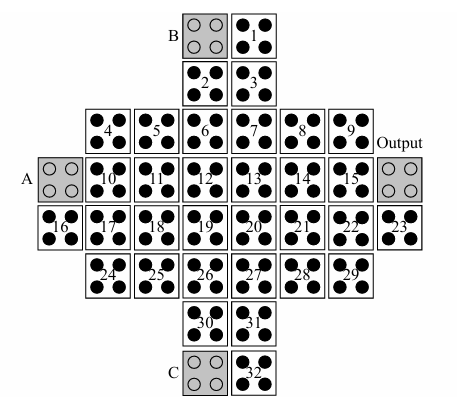
\includegraphics[width=\linewidth]{wang_vrata.png}
    \small (a) Osnovna struktura
\end{minipage}\hfill
\begin{minipage}[t]{0.32\textwidth}
    \centering
    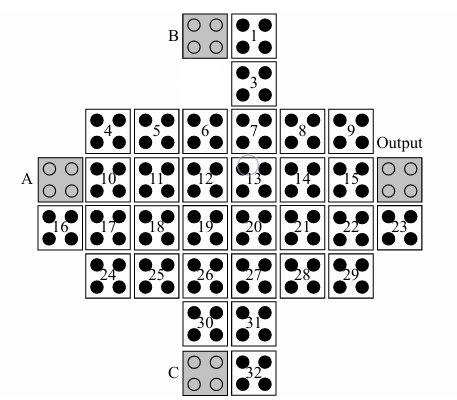
\includegraphics[width=\linewidth]{wang_vrata_brez2.png}
    \small (b) Brez celice 2
\end{minipage}\hfill
\begin{minipage}[t]{0.32\textwidth}
    \centering
    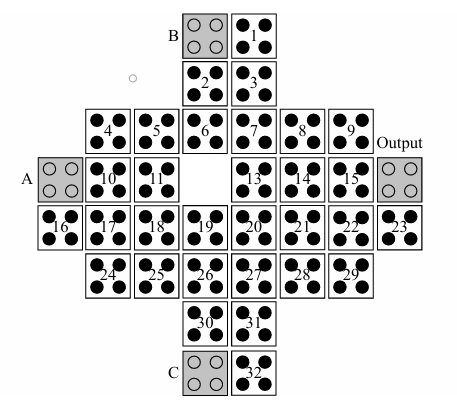
\includegraphics[width=\linewidth]{wang_vrata_brez12.png}
    \small (c) Brez celice 12
\end{minipage}
\caption{Struktura Wangovih večinskih vrat in prikaz konfiguracij z odstranjeno celico 2 oziroma 12.}
\label{g18:fig:wang-struktura}
\end{figure}


Pri odmikanju izbranih notranjih celic 6, 18, 2 in 12 za $0{,}5$, $1$ oziroma $1{,}5$ nm v vseh štirih smereh
so vsi zabeleženi izhodi pravilni ($8/8$), vrednosti $|P_Y|$ pa ostajajo približno $0{,}979$.
Celotne meritve so navedene v tabelah~\ref{g18:tab:wang-notranje-6-18} in \ref{g18:tab:wang-notranje-2-12}.

\begin{table}[H]
    \centering

    \begin{minipage}{0.49\textwidth}
        \centering
        \resizebox{\linewidth}{!}{%
            \begin{tabular}{|c|c|c|c|c|}
                \hline
                Celica & Smer & Odmik (nm) & Pravilne kombinacije & $|P_Y|$ \\
                \hline
                6 & Desno & 0.5 & 8/8 & 9.79e-001 \\
                6 & Desno & 1.0 & 8/8 & 9.79e-001 \\
                6 & Desno & 1.5 & 8/8 & 9.79e-001 \\
                6 & Levo & 0.5 & 8/8 & 9.79e-001 \\
                6 & Levo & 1.0 & 8/8 & 9.79e-001 \\
                6 & Levo & 1.5 & 8/8 & 9.79e-001 \\
                6 & Gor & 0.5 & 8/8 & 9.79e-001 \\
                6 & Gor & 1.0 & 8/8 & 9.79e-001 \\
                6 & Gor & 1.5 & 8/8 & 9.79e-001 \\
                6 & Dol & 0.5 & 8/8 & 9.79e-001 \\
                6 & Dol & 1.0 & 8/8 & 9.79e-001 \\
                6 & Dol & 1.5 & 8/8 & 9.79e-001 \\
                \hline
            \end{tabular}
        }
    \end{minipage}
    \hfill
    \begin{minipage}{0.49\textwidth}
        \centering
        \resizebox{\linewidth}{!}{%
            \begin{tabular}{|c|c|c|c|c|}
                \hline
                Celica & Smer & Odmik (nm) & Pravilne kombinacije & $|P_Y|$ \\
                \hline
                18 & Desno & 0.5 & 8/8 & 9.79e-001 \\
                18 & Desno & 1.0 & 8/8 & 9.79e-001 \\
                18 & Desno & 1.5 & 8/8 & 9.79e-001 \\
                18 & Levo & 0.5 & 8/8 & 9.79e-001 \\
                18 & Levo & 1.0 & 8/8 & 9.79e-001 \\
                18 & Levo & 1.5 & 8/8 & 9.79e-001 \\
                18 & Gor & 0.5 & 8/8 & 9.79e-001 \\
                18 & Gor & 1.0 & 8/8 & 9.79e-001 \\
                18 & Gor & 1.5 & 8/8 & 9.79e-001 \\
                18 & Dol & 0.5 & 8/8 & 9.79e-001 \\
                18 & Dol & 1.0 & 8/8 & 9.79e-001 \\
                18 & Dol & 1.5 & 8/8 & 9.79e-001 \\
                \hline
            \end{tabular}
        }
    \end{minipage}

    \caption{Rezultati majhnih geometrijskih odmikov notranjih celic 6 in 18 Wangovih vrat.}
    \label{g18:tab:wang-notranje-6-18}
\end{table}

\begin{table}[H]
    \centering

    \begin{minipage}{0.49\textwidth}
        \centering
        \resizebox{\linewidth}{!}{%
            \begin{tabular}{|c|c|c|c|c|}
                \hline
                Celica & Smer & Odmik (nm) & Pravilne kombinacije & $|P_Y|$ \\
                \hline
                2 & Desno & 0.5 & 8/8 & 9.79e-001 \\
                2 & Desno & 1.0 & 8/8 & 9.79e-001 \\
                2 & Desno & 1.5 & 8/8 & 9.79e-001 \\
                2 & Levo & 0.5 & 8/8 & 9.79e-001 \\
                2 & Levo & 1.0 & 8/8 & 9.79e-001 \\
                2 & Levo & 1.5 & 8/8 & 9.79e-001 \\
                2 & Gor & 0.5 & 8/8 & 9.79e-001 \\
                2 & Gor & 1.0 & 8/8 & 9.79e-001 \\
                2 & Gor & 1.5 & 8/8 & 9.79e-001 \\
                2 & Dol & 0.5 & 8/8 & 9.79e-001 \\
                2 & Dol & 1.0 & 8/8 & 9.79e-001 \\
                2 & Dol & 1.5 & 8/8 & 9.79e-001 \\
                \hline
            \end{tabular}
        }
    \end{minipage}
    \hfill
    \begin{minipage}{0.49\textwidth}
        \centering
        \resizebox{\linewidth}{!}{%
            \begin{tabular}{|c|c|c|c|c|}
                \hline
                Celica & Smer & Odmik (nm) & Pravilne kombinacije & $|P_Y|$ \\
                \hline
                12 & Desno & 0.5 & 8/8 & 9.79e-001 \\
                12 & Desno & 1.0 & 8/8 & 9.79e-001 \\
                12 & Desno & 1.5 & 8/8 & 9.79e-001 \\
                12 & Levo & 0.5 & 8/8 & 9.79e-001 \\
                12 & Levo & 1.0 & 8/8 & 9.79e-001 \\
                12 & Levo & 1.5 & 8/8 & 9.79e-001 \\
                12 & Gor & 0.5 & 8/8 & 9.79e-001 \\
                12 & Gor & 1.0 & 8/8 & 9.79e-001 \\
                12 & Gor & 1.5 & 8/8 & 9.79e-001 \\
                12 & Dol & 0.5 & 8/8 & 9.79e-001 \\
                12 & Dol & 1.0 & 8/8 & 9.79e-001 \\
                12 & Dol & 1.5 & 8/8 & 9.79e-001 \\
                \hline
            \end{tabular}
        }
    \end{minipage}

    \caption{Rezultati majhnih geometrijskih odmikov notranjih celic 2 in 12 Wangovih vrat.}
    \label{g18:tab:wang-notranje-2-12}
\end{table}

Izkaže se, da tudi večji odmiki robnih celic ne povzročajo napak v delovanju Wangovih vrat, saj so rezultati pravilni ($8/8$) in je absolutna izhodna polarizacija še vedno približno $0{,}979$.
Izvedli smo premike celic 2, 3 in 24 za $10$ nm v smeri, kamor to struktura dopušča, ter so bili rezultati še vedno pravilni.

\subsubsection{Premiki vhodnih celic}

Pri večjih odmikih vhodnih celic so se pojavile nepravilnosti, čeprav je navedena absolutna vrednost
polarizacije v tabeli~\ref{g18:tab:wang-vhodi} ostala približno $0{,}979$.
Pri vhodu $A$ je denimo premik levo za $10$ nm povzročil rezultat $4/8$, premik gor za $20$ nm
pa ponovno $8/8$. Pri vhodih $B$ in $C$ se za nekatere odmike rezultat zmanjša na $6/8$.
Tabela vključuje izbrane preizkušene odmike, ne celotnega zveznega območja.

\begin{table}[H]
    \centering
    \begin{minipage}{0.49\textwidth}
        \centering
        \resizebox{\linewidth}{!}{%
            % TABELA CELICA 6
            \begin{tabular}{|c|c|c|c|c|}
                \hline
                Celica & Smer & Odmik (nm) & Pravilne kombinacije & $|P_Y|$ \\
                \hline
                A & Levo & 10 & 4/8 & 9.79e-001 \\
                A & Gor & 7 & 4/8 & 9.79e-001 \\
                A & Gor & 20 & 8/8 & 9.79e-001 \\
                A & Diagonalno & 19 & 6/8 & 9.79e-001 \\
                \hline
            \end{tabular}
        }
    \end{minipage}
    \hfill
    \begin{minipage}{0.49\textwidth}
        \centering
        \resizebox{\linewidth}{!}{%
            \begin{tabular}{|c|c|c|c|c|}
                \hline
                Celica & Smer & Odmik (nm) & Pravilne kombinacije & $|P_Y|$ \\
                \hline
                B & Levo & 7 & 7/8 & 9.79e-001 \\
                B & Levo & 7.5 & 6/8 & 9.79e-001 \\
                B & Levo & 8 & 6/8 & 9.79e-001 \\
                B & Gor & 7.5 & 6/8 & 9.79e-001 \\
                B & Gor & 8 & 6/8 & 9.79e-001 \\
                B & Diagonalno & 6 & 6/8 & 9.79e-001 \\
                \hline
            \end{tabular}
        }
    \end{minipage}
    \vspace{1cm}
    \begin{minipage}{0.49\textwidth}
        \centering
        \resizebox{\linewidth}{!}{%
            \begin{tabular}{|c|c|c|c|c|}
                \hline
                Celica & Smer & Odmik (nm) & Pravilne kombinacije & $|P_Y|$ \\
                \hline
                C & Levo & 7.5 & 6/8 & 9.79e-001 \\
                C & Levo & 8 & 6/8 & 9.79e-001 \\
                C & Dol & 8 & 6/8 & 9.79e-001 \\
                C & Diagonalno & 6 & 6/8 & 9.79e-001 \\
                \hline
            \end{tabular}
        }
    \end{minipage}
    \caption{Izbrani odmiki vhodnih celic $A$, $B$ in $C$ pri Wangovih vratih.}
    \label{g18:tab:wang-vhodi}
\end{table}

\subsubsection{Premiki izhodne celice}
\label{g18:sec:rez-wang-y}

Najizrazitejše spremembe v izhodni polarizaciji in pravilnosti smo pri Wangovih vratih opazili pri premikih
izhodne celice $Y$. V tabeli~\ref{g18:tab:wang-izhod} so prikazani vsi izmerjeni premiki desno in navzgor, saj nam struktura omogoča te premike.

\begin{table}[H]
    \centering
    \begin{minipage}{0.49\textwidth}
        \centering
        \resizebox{\linewidth}{!}{%
            \begin{tabular}{|c|c|c|c|}
                \hline
                Smer & Odmik (nm) & Pravilne kombinacije & $|P_Y|$ \\
                \hline
                Desno & 2 & 8/8 & 9.65e-001 \\
                Desno & 4 & 8/8 & 9.24e-001 \\
                Desno & 6 & 8/8 & 7.55e-001 \\
                Desno & 7 & 8/8 & 5.12e-001 \\
                Desno & 8 & 8/8 & 1.37e-001 \\
                Desno & 8.5 & 0/8 & 6.03e-002 \\
                Desno & 9 & 0/8 & 2.34e-001 \\
                Desno & 9.5 & 0/8 & 3.75e-001 \\
                Desno & 10 & 0/8 & 4.82e-001 \\
                Desno & 12 & 0/8 & 6.76e-001 \\
                Desno & 14 & 0/8 & 7.08e-001 \\
                Desno & 16 & 0/8 & 6.73e-001 \\
                Desno & 18 & 0/8 & 5.97e-001 \\
                \hline
            \end{tabular}
        }
    \end{minipage}
    \hfill
    \begin{minipage}{0.49\textwidth}
        \centering
        \resizebox{\linewidth}{!}{%
            \begin{tabular}{|c|c|c|c|}
                \hline
                Smer & Odmik (nm) & Pravilne kombinacije & $|P_Y|$ \\
                \hline
                Gor & 2 & 8/8 & 9.58e-001 \\
                Gor & 4 & 8/8 & 8.74e-001 \\
                Gor & 5 & 8/8 & 7.23e-001 \\
                Gor & 5.5 & 8/8 & 5.64e-001 \\
                Gor & 6 & 8/8 & 3.16e-001 \\
                Gor & 7 & 0/8 & 2.93e-001 \\
                Gor & 8 & 0/8 & 6.14e-001 \\
                Gor & 9 & 0/8 & 7.31e-001 \\
                Gor & 10 & 0/8 & 7.66e-001 \\
                Gor & 11 & 0/8 & 7.48e-001 \\
                Gor & 12 & 0/8 & 6.63e-001 \\
                Gor & 14 & 0/8 & 6.63e-001 \\
                Gor & 16 & 8/8 & 7.45e-001 \\
                Gor & 18 & 8/8 & 9.02e-001 \\
                Gor & 20 & 8/8 & 9.32e-001 \\
                Gor & 22 & 8/8 & 9.23e-001 \\
                Gor & 24 & 8/8 & 8.62e-001 \\
                Gor & 26 & 8/8 & 5.98e-001 \\
                Gor & 27 & 8/8 & 2.60e-001 \\
                Gor & 28 & 0/8 & 1.74e-001 \\
                \hline
            \end{tabular}
        }
    \end{minipage}
    \caption{Pravilnost in absolutna polarizacija pri premikanju izhodne celice $Y$ Wangovih vrat.}
    \label{g18:tab:wang-izhod}
\end{table}


\subsubsection{Analiza rezultatov Wangovih večinskih vrat}
\label{g18:sec:rez-wang-analiza}

Rezultati simulacij kažejo na to, da so Wangova večinska vrata razmeroma odporna na majhne premike notranjih celic, saj so ohranila pravilno delovanje ($8/8$) pri vseh premikih, izhodna polarizacija pa se ni spremenila. 
Podobno smo opazili tudi na večjih izbranih premikih robnih celic strukture.

Večjo občutljivost smo opazili pri premikih vhodnih celic. Pri nekaterih premikih se je delovanje zmanjšalo na $4/8$ oziroma $6/8$, čeprav je absolutna izhodna polarizacija ostala približno $0{,}979$. V posameznih primerih se je pravilno delovanje ponovno vzpostavilo tudi pri večjem premiku.
Rezultati tovrstnih premikov vhodne celice so pokazali, da se pravilnost delovanja vrat ne spreminja nujno monotono z velikostjo premika. Vhodne celice se namreč pri določenih premikih približujejo drugim celicam v strukturi, kar lahko povzroči spremembe elektrostatičnih interakcij in posledično vpliva na pravilnost delovanja vrat.

Zanimive rezultate pa smo dobili pri premikanju izhodne celice $Y$. Pri premikih v desno se je absolutna polarizacija postopoma zmanjševala in pri odmiku $8$ nm dosegla $|P_Y|=0{,}137$, čeprav so vrata še vedno pravilno izvedla vseh osem vhodnih kombinacij. Že pri odmiku $8{,}5$ nm se je pravilnost zmanjšala na $0/8$. Pri nadaljnjih premikih se je polarizacija ponovno povečevala, vendar se pravilno delovanje v preizkušenem območju ni vzpostavilo.
Na slikah \ref{g18:fig:wang-premik-desno} in \ref{g18:fig:wang-premik-gor} sta prikazani odvisnosti absolutne izhodne polarizacije in pravilnosti delovanja od velikosti premika izhodne celice $Y$ v desno in navzgor.

\begin{figure}[H]
    \centering
    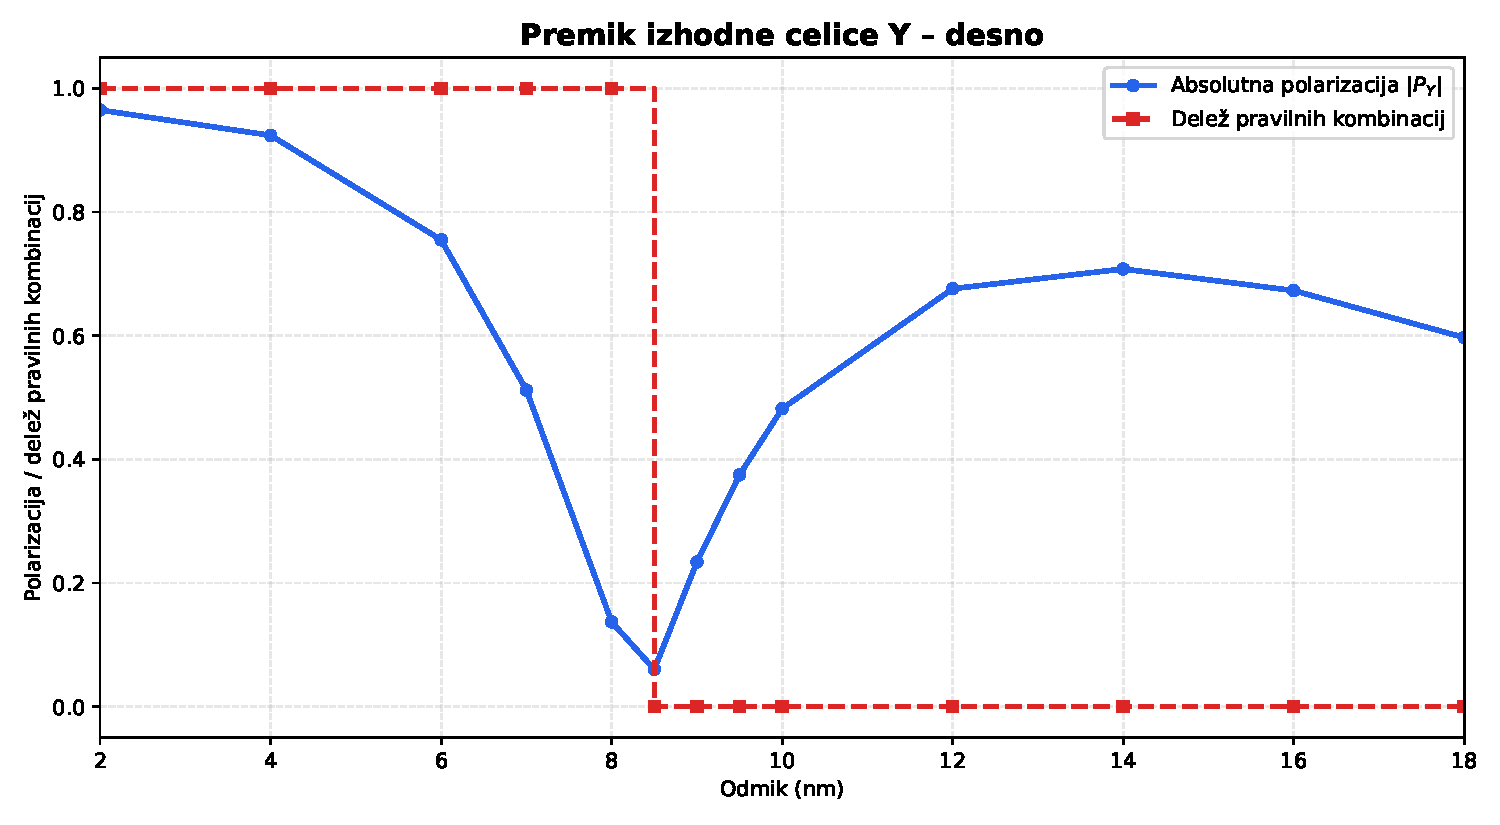
\includegraphics[width=0.85\textwidth]{Figure_1.pdf}
    \caption{Vpliv premika izhodne celice $Y$ v desno
    na absolutno polarizacijo in pravilnost delovanja
    Wangovih večinskih vrat.}
    \label{g18:fig:wang-premik-desno}
\end{figure}
\begin{figure}[H]
    \centering
    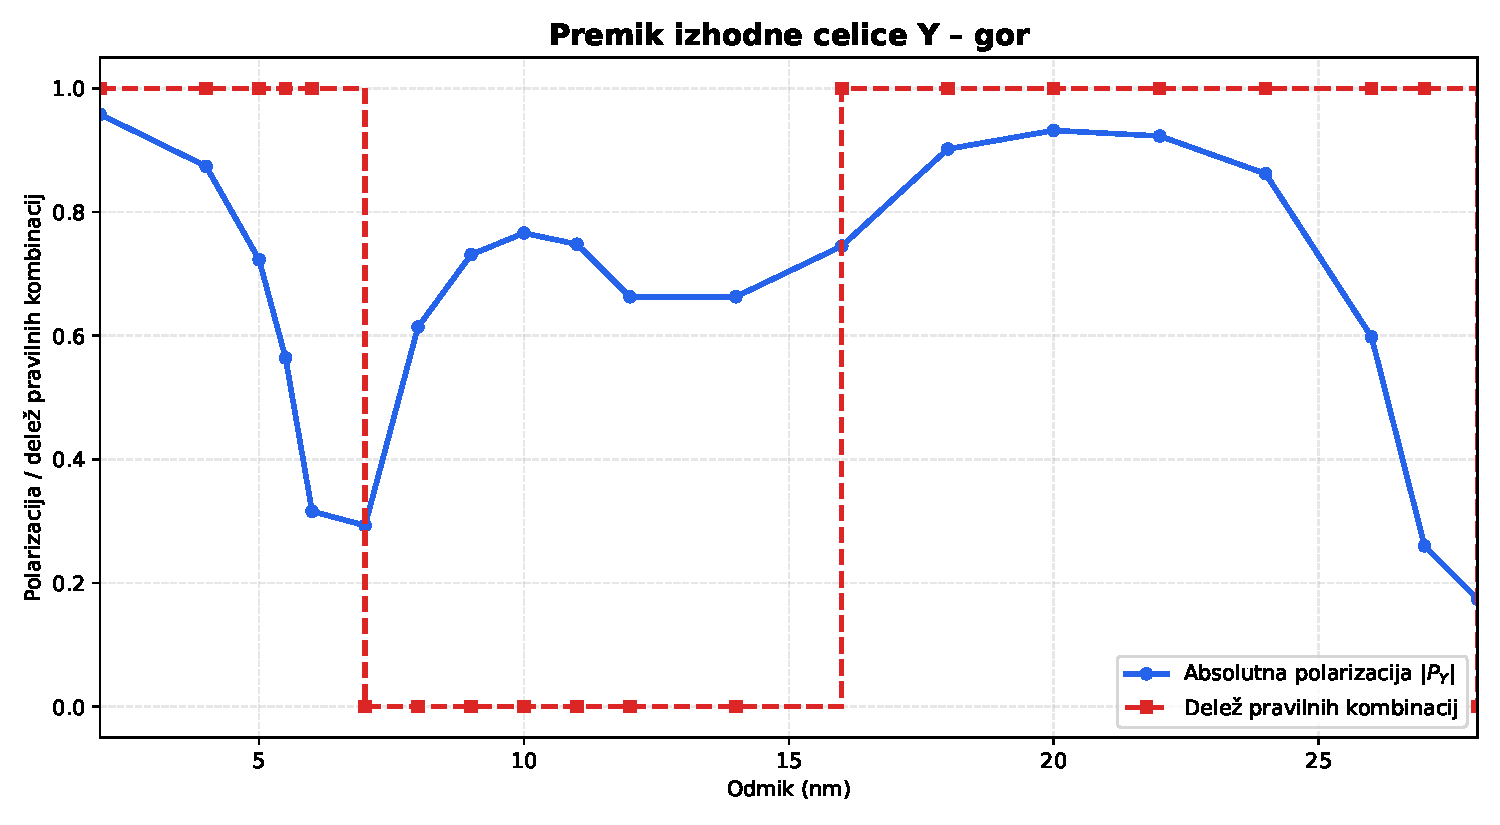
\includegraphics[width=0.85\textwidth]{Figure_2.pdf}
    \caption{Vpliv premika izhodne celice $Y$ navzgor
    na absolutno polarizacijo in pravilnost delovanja
    Wangovih večinskih vrat.}
    \label{g18:fig:wang-premik-gor}
\end{figure}
Opazimo, da so spremembe pri premikih navzgor in desno različne. Pri premikih navzgor smo opazili še izrazitejše spremembe. Do odmika $6$ nm so vrata delovala pravilno, med $7$ in $14$ nm pa je pravilnost padla na $0/8$. Pri odmikih med $16$ in $27$ nm se je pravilno delovanje ponovno vzpostavilo ($8/8$), pri odmiku $28$ nm pa smo znova zabeležili $0/8$.
Zaradi kompleksnosti rezultatov je težko napovedati, kako se bo pravilnost delovanja spremenila pri določenem premiku celice. Vpliv velikosti odmika ni bil vedno predvidljiv, saj se je v nekaterih primerih pravilno delovanje ponovno vzpostavilo tudi pri večjih odmikih. Takšno obnašanje je lahko posledica spreminjanja elektrostatičnih interakcij, saj se premaknjena celica približuje drugim celicam v strukturi oziroma se od njih oddaljuje.


\subsection{Vpliv geometrijskih odmikov na elektrostatične interakcije in delovanje večinskih vrat}
\label{g18:sec:rez-energija}

\subsubsection{Elektrostatična energija in \emph{kink energy}}
\label{g18:sec:elektrostaticna-energija}

Geometrijski odmiki vplivajo na elektrostatične interakcije med celicami. Energijo prevoja (\emph{kink energy}) definiramo kot razliko energij nasprotnih in enakih polarizacij:

\begin{equation}
    E_{\mathrm{kink}} =
    E_{\mathrm{opposite}} - E_{\mathrm{same}}.
\end{equation}

Interakcijsko energijo dveh celic izračunamo s Coulombovim zakonom:

\begin{equation}
    E_{}^{ij} =
    \frac{1}{4\pi\varepsilon_0\varepsilon_r}
    \sum_{n=1}^{4}\sum_{m=1}^{4}
    \frac{q_{n}^{i}q_{m}^{j}}{|r_{n}^{i}-r_{m}^{j}|}.
\end{equation}

Tu sta $q$ in $r$ naboj ter položaj kvantne pike, $\varepsilon_0$ in $\varepsilon_r$ pa dielektričnost vakuuma in relativna dielektričnost. Izpise $E_k$ v QCADesigner-E uporabimo kot parne interakcijske koeficiente $K_{ij}$ za primerjavo odmikov.

\subsubsection{Rezultati simulacij interakcijskih koeficientov}
\label{g18:sec:interakcijski-koeficienti}

Notranjo celico smo premikali za 0,5, 1, 1,5 in 2 nm v vseh štirih smereh, pri nespremenjenih preostalih celicah in simulacijskih nastavitvah. Pri 2 nm se robova sosednjih celic stikata. Iz energijskih izpisov smo odčitali koeficiente povezav med notranjo celico ter celicami $A$, $B$, $C$ in $Y$ (tabeli~\ref{g18:tab:energija-vodoravno} in~\ref{g18:tab:energija-navpicno}).

\noindent Brez odmika: $K_A$ = $K_B$ = $K_C$ = $K_Y$ = 1.484 meV

\begin{table}[H]
    \centering
    \caption{Interakcijski koeficienti pri vodoravnih premikih
    notranje celice.}
    \label{g18:tab:energija-vodoravno}
    \begin{tabular}{cccccc}
        \toprule
        Smer &  Odmik [nm] & $K_A$ [meV] & $K_B$ [meV] & $K_C$ [meV] & $K_Y$ [meV] \\
        \midrule
        Levo & 0.5 & 1.474 & 1.687 & 1.474 & 1.309 \\
        Levo & 1.0 & 1.446 & 1.926 & 1.446 & 1.158 \\
        Levo & 1.5 & 1.400 & 2.205 & 1.400 & 1.027 \\
        Levo & 2.0 & 1.337 & 2.535 & 1.337 & 0.914 \\
        \midrule
        Desno & 0.5 & 1.474 & 1.309 & 1.474 & 1.687 \\
        Desno & 1.0 & 1.446 & 1.158 & 1.446 & 1.926 \\
        Desno & 1.5 & 1.400 & 1.027 & 1.400 & 2.205 \\
        Desno & 2.0 & 1.337 & 0.914 & 1.337 & 2.535 \\
        \bottomrule
    \end{tabular}
\end{table}

\begin{table}[H]
    \centering
    \caption{Interakcijski koeficienti pri navpičnih
    odmikih notranje celice.}
    \label{g18:tab:energija-navpicno}
    \begin{tabular}{cccccc}
        \toprule
        Smer & Odmik [nm] & $K_A$ [meV] & $K_B$ [meV] & $K_C$  [meV] & $K_Y$  [meV] \\
        \midrule
        Gor & 0.5 & 1.687 & 1.474 & 1.309 & 1.474 \\
        Gor & 1.0 & 1.926 & 1.446 & 1.158 & 1.446 \\
        Gor & 1.5 & 2.205 & 1.400 & 1.027 & 1.400 \\
        Gor & 2.0 & 2.535 & 1.337 & 0.914 & 1.337 \\
        \midrule
        Dol & 0.5 & 1.309 & 1.474 & 1.687 & 1.474 \\
        Dol & 1.0 & 1.158 & 1.446 & 1.926 & 1.446 \\
        Dol & 1.5 & 1.027 & 1.400 & 2.205 & 1.400 \\
        Dol & 2.0 & 0.914 & 1.337 & 2.535 & 1.337 \\
        \bottomrule
    \end{tabular}
\end{table}

Interakcija s celico v smeri premika se povečuje, z nasprotno pa zmanjšuje. Pri 1,5 nm v levo se $K_B$ poveča z 1,484 na 2,205 meV (+48,7\,\%), $K_Y$ pa zmanjša na 1,027 meV ($-30,8\,\%$). Pri navpičnih premikih se $K_A$ in $K_C$ spreminjata zrcalno. Pri 2 nm koeficient v smeri premika doseže 2,535 meV (+70,9\,\%). Trende prikazujeta sliki \ref{g18:fig:odmik-vodoravno} in \ref{g18:fig:odmik-navpicno}.

\begin{figure}[H]
    \centering

    \begin{subfigure}[t]{0.49\textwidth}
        \centering
        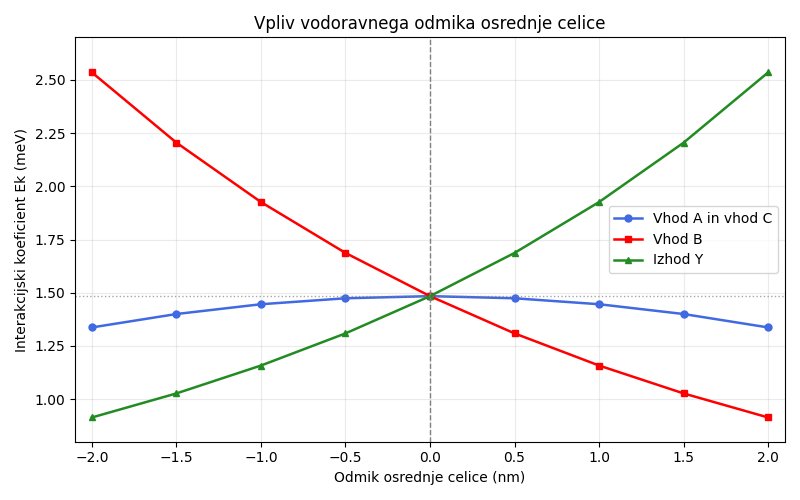
\includegraphics[width=\linewidth]{Figure_3.png}
        \caption{Vodoravni odmik}
        \label{g18:fig:odmik-vodoravno}
    \end{subfigure}
    \hfill
    \begin{subfigure}[t]{0.49\textwidth}
        \centering
        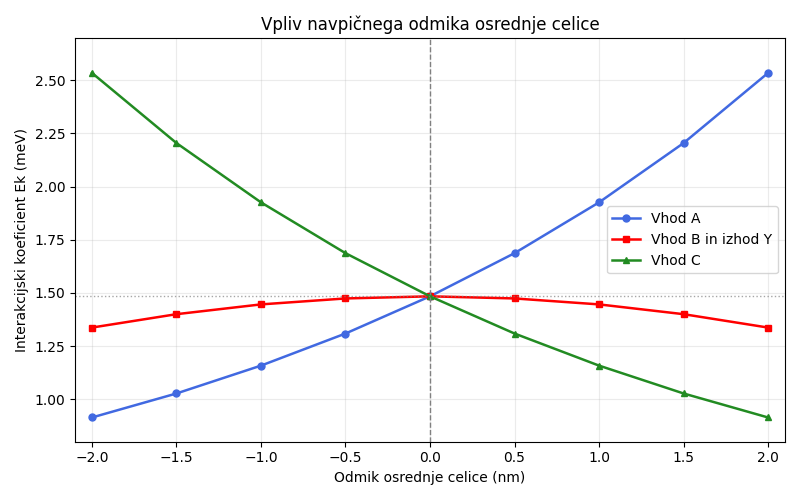
\includegraphics[width=\linewidth]{Figure_4.png}
        \caption{Navpični odmik}
        \label{g18:fig:odmik-navpicno}
    \end{subfigure}

    \caption{Vpliv geometrijskih odmikov notranje celice na interakcijske koeficiente s sosednjimi celicami.}
    \label{g18:fig:odmiki-interakcije}
\end{figure}

\subsubsection{Povezava elektrostatičnih interakcij z delovanjem večinskih vrat}
\label{g18:sec:povezava-interakcij}

V simetrični postavitvi so vplivi vhodov na notranjo celico enakovredni. Po odmiku polarizacijo približno ocenimo z uteženo vsoto
\begin{equation}
    S=K_AP_A+K_BP_B+K_CP_C,\qquad P_M\approx\operatorname{sgn}(S),
\end{equation}
kjer so $P_A,P_B,P_C\in\{-1,+1\}$ vhodne polarizacije, $K_A,K_B,K_C>0$ pa interakcijski koeficienti iz QCADesigner-E. Model ne upošteva izhodne celice in časovne dinamike vezja.

Za vhodno kombinacijo $(P_A,P_B,P_C)=(+1,-1,-1)$ in odmik notranje celice za 2 nm navzgor dobimo
\[
    S=2.535-1.337-0.914=+0.284\,\mathrm{meV}.
\]
Model napove $P_M=+1$, čeprav je pravilna večinska vrednost $-1$, saj bližji vhod $A$ prevlada nad drugima. Analogno lahko pri odmiku navzdol prevlada vhod $C$. Pri 2 nm v levo je sicer $K_B$ največji, vendar $K_B=2{,}535<K_A+K_C=2{,}674$ meV. Poenostavljeni model zato ne pojasni simuliranih napak 6/8. Pri premiku v desno se okrepi predvsem sklopitev z izhodom $Y$, ki v modelu ni upoštevana.

\subsubsection{Elektrostatični izračun in primerjava modelov}
\label{g18:sec:primerjava-modelov}

Po vzoru Dhare in Mehta~\cite{g18:dhare2023} za vhodno kombinacijo $(+1,-1,-1)$ izračunamo Coulombove energije pri odmikih notranje celice za 0, 1 in 2 nm navzgor. Uporabimo poenostavljeno geometrijo iz tabele~\ref{g18:tab:parametri-qca}, ki ni nujno enaka notranjemu modelu QCADesigner-E.

\begin{table}[H]
    \centering
    \begin{minipage}[t]{0.55\linewidth}
        \centering
        \captionof{table}{Geometrijski in fizikalni parametri modela QCA celic.}
        \label{g18:tab:parametri-qca}
        \vspace{2pt}
        \resizebox{\linewidth}{!}{%
        \begin{tabular}{lc}
            \toprule
            Parameter & Vrednost \\
            \midrule
            Širina celice & 18 nm \\
            Višina celice & 18 nm \\
            Razmik med celicama & 2 nm \\
            Razdalja med središčema sosednjih celic & 20 nm \\
            Premer kvantne pike & 5 nm \\
            Razdalja med središči kvantnih pik & 9 nm \\
            Relativna dielektričnost $\varepsilon_r$ & 12,9 \\
            \bottomrule
        \end{tabular}}
    \end{minipage}\hfill
    \begin{minipage}[t]{0.42\linewidth}
        \centering
        \captionof{table}{Razdalja $A$--$M$ in koeficient $K_A$ pri odmikih navzgor.}
        \label{g18:tab:izbrani-odmiki}
        \vspace{2pt}
        \resizebox{\linewidth}{!}{%
        \begin{tabular}{ccc}
            \toprule
            Odmik [nm] & Razdalja $A$--$M$ [nm] & $K_A$ [meV] \\
            \midrule
            0 & 20 & 1.484 \\
            1 & 19 & 1.926 \\
            2 & 18 & 2.535 \\
            \bottomrule
        \end{tabular}}
    \end{minipage}
\end{table}

\paragraph{Postopek izračuna.}

Izhodišče koordinatnega sistema postavimo v središče nepremaknjene notranje celice. Središča vhodov so $A=(0,20)$, $B=(-20,0)$ in $C=(0,-20)$ nm, notranja celica pa ima pri odmiku $d$ navzgor središče $M=(0,d)$ nm. Relativne koordinate kvantnih pik so
\[
\begin{aligned}
q_1 &= (-4.5, 4.5),  & q_2 &= (4.5, 4.5), \\
q_3 &= (4.5, -4.5), & q_4 &= (-4.5, -4.5)
\end{aligned}
\qquad \mathrm{[nm]}
\]
Pri $P=+1$ sta zasedeni piki $q_1,q_3$, pri $P=-1$ pa $q_2,q_4$. Za ponazoritev: pri $d=2$ nm in $P_A=P_M=+1$ sta elektrona v pikah $A_1=(-4.5,24.5)$ nm in $M_1=(-4.5,6.5)$ nm oddaljena $18$ nm.

Za vsako izbrano polarizacijo $P_M$ seštejemo štiri interakcije med notranjo celico in vsakim od treh vhodov, skupaj torej 12 členov:
\begin{equation}
E(P_M)=\sum_{X\in\{A,B,C\}}\sum_{i\in D_X}\sum_{j\in D_M}
\frac{e^2}{4\pi\varepsilon_0\varepsilon_r\,r_{ij}},\qquad
r_{ij}=\sqrt{(x_i-x_j)^2+(y_i-y_j)^2}.
\end{equation}
Množici $D_X$ in $D_M$ vsebujeta položaja dveh zasedenih pik posamezne celice. Vse razdalje in energije za obe možnosti $P_M\in\{-1,+1\}$ smo izračunali v Pythonu.

\paragraph{Rezultati in primerjava.}

Definiramo $\Delta E=E(+1)-E(-1)$. Pozitivna razlika daje prednost $P_M=-1$, negativna pa $P_M=+1$. Izračunane vrednosti so v tabeli \ref{g18:tab:izracun-energij}.

\begin{table}[H]
    \centering
    \caption{Izračunane elektrostatične energije
    in napovedana polarizacija notranje celice
    pri izbranih odmikih navzgor.}
    \label{g18:tab:izracun-energij}
    \begin{tabular}{ccccc}
        \toprule
        Odmik [nm] &
        $E(+1)$ [meV] &
        $E(-1)$ [meV] &
        $\Delta E$ [meV] &
        $P_M$ \\
        \midrule
        0 & 71.045 & 69.561 & +1.484 & $-1$ \\
        1 & 70.764 & 70.399 & +0.365 & $-1$ \\
        2 & 70.657 & 71.563 & -0.906 & $+1$ \\
        \bottomrule
    \end{tabular}
\end{table}

Pri 0 in 1 nm je energijsko ugodnejša pravilna polarizacija $-1$, pri 2 nm pa se predznak $\Delta E$ obrne. Z vrednostjo $S=K_A-K_B-K_C$ primerjamo obe matematični napovedi ter pravilnost celotnih vrat iz simulacij (tabela~\ref{g18:tab:primerjava-modelov}).

\begin{table}[H]
    \centering
    \caption{Primerjava matematičnih napovedi za vhodno kombinacijo $(+1,-1,-1)$ in števila pravilnih izhodnih kombinacij v simulaciji (od vseh osmih).}
    \label{g18:tab:primerjava-modelov}
    \small
    \resizebox{\linewidth}{!}{%
    \begin{tabular}{cccccc}
        \toprule
        Odmik [nm] &
        $S$ [meV] &
        $\Delta E$ [meV] &
        $P_M$ (stat.) &
        $P_M$ (elektr.) &
        Pravilne kombinacije \\
        \midrule
        0 & -1.484 & +1.484 & $-1$ & $-1$ & 8/8 \\
        1 & -0.678 & +0.365 & $-1$ & $-1$ & 8/8 \\
        2 & +0.284 & -0.906 & $+1$ & $+1$ & 6/8 \\
        \bottomrule
    \end{tabular}}
\end{table}

Oba modela napovesta enak predznak $P_M$, vendar $S$ in $\Delta E$ nista ista fizikalna količina. Simulacija pri 2 nm pokaže 6/8 pravilnih izhodov, kar podpira splošni trend, ne dokazuje pa, da je napačna prav kombinacija $(+1,-1,-1)$: za to bi morali posebej odčitati njen izhodni signal.

\subsubsection{Ugotovitve}
\label{g18:sec:energijske-ugotovitve}
Geometrijski odmiki spremenijo razmerje med elektrostatičnimi interakcijami in lahko povzročijo napačno večinsko odločitev. Pri odmiku 2 nm navzgor oba statična modela napovesta napačno polarizacijo notranje celice, simulacija pa pokaže 6/8 pravilnih izhodov. Modela tako pojasnjujeta možen vzrok napak, vendar ne nadomeščata dinamične simulacije.

\newpage


\section{Razprava}
\label{g18:sec:razprava}

Rezultati kažejo, da na pravilnost delovanja večinskih vrat vplivajo velikost, smer in položaj geometrijskega odmika.
Pri osnovnih petceličnih vratih lahko že manjši premiki osrednje celice povzročijo napake, Wangova vrata pa so
pri preizkušenih premikih notranjih celic odpornejša. Pri obeh strukturah smo opazili, da pravilnost delovanja
ni vedno monotono odvisna od velikosti odmika. 
S tem smo potrdili le del začetnih pričakovanj, saj večji odmik ne pomeni nujno večjega števila napak, ter so lahko rezultati nepredvivljivi.
Matematična analiza je pokazala, da lahko geometrijski odmiki spremenijo razmerje elektrostatičnih interakcij med celicami, kar lahko povzroči napačno večinsko odločitev.


\subsection{Kaj ni delovalo}
\label{g18:sec:neuspehi}

Pri nekaterih odmikih so vrata delovala nepravilno kljub visoki absolutni izhodni polarizaciji.
Poleg tega poenostavljeni energijski model ni pojasnil vseh napak, opaženih pri simulacijah, saj ne upošteva celotne dinamike vezja.
Poenostavljeni energijski model ni uspel pojasniti vseh rezultatov simulacij. Pri premiku osrednje celice za $2$ nm v levo ni napovedal napak, ki smo jih opazili v QCADesigner-E. To kaže na omejitve modela, ki ne upošteva vseh interakcij in časovne dinamike vezja.

\section{Zaključek}
\label{g18:sec:zakljucek}

Z analizo smo pokazali, da geometrijski odmiki pomembno vplivajo na pravilnost in polarizacijo večinskih vrat.
Wangova vrata so bila pri preizkušenih premikih notranjih celic razmeroma odporna, medtem ko so se pri vhodnih in izhodni celici pojavile izrazitejše spremembe.
Energijska analiza osnovnih vrat je dodatno pomagala pojasniti vpliv odmikov na elektrostatične interakcije.

Raziskavo bi lahko nadaljevali z analizo več hkratnih odmikov celic in preverjanjem delovanja pri različnih simulacijskih nastavitvah.


\section*{Doprinosi avtorjev}

Teja Blažič: [Pregled teoretičnih osnov, implementacija osnovnih večinskih vrat, izvedba simulacij geometrijskih odmikov in matematična analiza.]

Nejc Čeh: [ Pregled alternativnih večinskih vrat, implementacija strukture, primerjalne simulacije in analiza odpornosti na napake.]


\section*{Izjava o uporabi generativne umetne inteligence}

Pri pripravi seminarske naloge smo uporabili orodje ChatGPT kot pomoč pri iskanju ustrezne strokovne literature,
jezikovnem urejanju in oblikovanju besedila ter pripravi programske kode za izris grafov. V manjši meri smo ga
uporabili tudi za pomoč matematičnega ozadja obravnavanih interakcij.
Simulacije, zbiranje podatkov, analiza rezultatov in končne ugotovitve so rezultat našega samostojnega dela.


\begin{thebibliography}{9}

\bibitem{g18:wang2018}
X. Wang, G. Xie, F. Deng, Y. Quan in H. Lü,
\textit{Design and comparison of new fault-tolerant
majority gate based on quantum-dot cellular automata},
Journal of Semiconductors, 39(8), 085001, 2018.

\url{https://doi.org/10.1088/1674-4926/39/8/085001}

\bibitem{g18:dhare2023}
V. Dhare in U. Mehta,
\textit{Analytical method for cell displacement defect
quantum-dot cellular automata primitive},
Journal of Electronic Science and Technology,
21(1), 100183, 2023.

\url{https://www.sciencedirect.com/science/article/pii/S1674862X23000010}

\end{thebibliography}


\end{document}

